\begin{enumerate}
\item In Fig \ref{figure_2}, $PQ$ is a tangent at point $C$ to a circle with centre $O$. If $AB$ is a diameter and $\angle CAB = 30\degree $, Find $\angle PCA$.\\
\begin{figure}[H]
\centering
	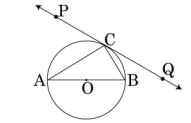
\includegraphics[width=5cm]{figs/2016_10_1.png}
	\caption{}
\label{figure_2}
\end{figure} 
\item  In Fig \ref{figure_3}, a quadrilateral $ABCD$ is drawn to circumscribe a circle, with centre $O$, in such a way that the sides $AB, BC, CD$ and $DA$ touch the circle at the points $P, Q, R$ and $S$ respectively. Prove that $ AB + CD= BC + DA $.\\
	\begin{figure}[H]
\centering
      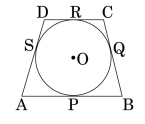
\includegraphics[width=5cm]{figs/2016_10_2.png}
      \caption{}
      \label{figure_3}
\end{figure} 
\item  In Fig \ref{figure_4}, from an external point $P$, two tangents $PT$ and $PS$ are drawn to a circle with centre $O$ and radius $r$. If $OP = 2r$, show that $\angle OTS = \angle OST= 30\degree$.
\begin{figure}[H]
\centering
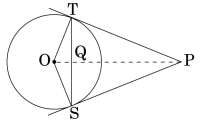
\includegraphics[width=5cm]{figs/2016_10_3.png}
\caption{}
      \label{figure_4}
   \end{figure} 
 \item  In fig \ref{figure_5}, $O$ is the centre of a circle such that diameter $AB = 13$ cm and $AC = 12$ cm. $BC$ is joined. Find the area of the shaded region. (Take $\pi = 3.14$)\\

	\begin{figure}[H]
      \centering
      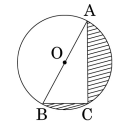
\includegraphics[width=5cm]{figs/2016_10_4.png}
      \caption{}
      \label{figure_5}
\end{figure} 
\item In Fig \ref{figure_6} , two equal circles, with centres $O$ and $O^\prime$, touch each other at $X$.$OO\prime$ produced meets the circle with centre $O^\prime$ at $A$. $AC$ is tangent to the circle with centre $O$, at the point $C$. $O^\prime D$ is perpendicular to $AC$. Find the value of $\dfrac{DO^\prime}{CO^\prime}$.\\
	\begin{figure}[H]
      \centering
      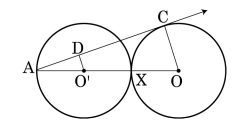
\includegraphics[width=5cm]{figs/2016_10_7.png}
      \caption{}
      \label{figure_6}
   \end{figure} 
 
\item Prove that the lengths of the tangents drawn from an external point to a circle are equal.

\end{enumerate}
